% CALCULATIONS.TEX
%
% The documentation in this file is part of PyXPlot <http://www.pyxplot.org.uk>
%
% Copyright (C) 2006-2010 Dominic Ford <coders@pyxplot.org.uk>
%               2008-2010 Ross Church
%
% $Id$
%
% PyXPlot is free software; you can redistribute it and/or modify it under the
% terms of the GNU General Public License as published by the Free Software
% Foundation; either version 2 of the License, or (at your option) any later
% version.
%
% You should have received a copy of the GNU General Public License along with
% PyXPlot; if not, write to the Free Software Foundation, Inc., 51 Franklin
% Street, Fifth Floor, Boston, MA  02110-1301, USA

% ----------------------------------------------------------------------------

% LaTeX source for the PyXPlot Users' Guide

\chapter{Performing Calculations}

The previous chapter described how PyXPlot can be used to plot data directly
from \datafile s onto graphs. Often, however, calculations need to be performed
on data before it is plotted. This chapter describes the mathematical
environment which PyXPlot provides for performing calculations either upon
single numerical values or upon whole datasets.  For simplicity, most of the
examples in this chapter will act upon single numerical values, displaying the
results using the {\tt print} command, thus using PyXPlot essentially as a
desktop calculator. In subsequent chapters, more examples will be given of the
use of PyXPlot's mathematical environment to analyse whole datasets and produce
plots.

\section{Variables}

Variables can be assigned to hold numerical values using syntax of the form:

\begin{verbatim} a = 5.2 * sqrt(64) \end{verbatim}

\noindent which may optionally be written as:\indcmd{let}

\begin{verbatim} let a = 5.2 * sqrt(64) \end{verbatim}

\noindent Numerical variables can subsequently be used by name in mathematical
expressions, as in the example:

\begin{verbatim} print a / sqrt(64) \end{verbatim}

\noindent Having been defined, variables can later be undefined -- set to have
no value -- using syntax of the form:

\begin{verbatim} a = \end{verbatim}

A list of all of the variables which are currently defined can be obtained by
typing {\tt show variables}\indcmd{show variables}. By default, an extensive
list is returned, as many physical constants are pre-defined by PyXPlot. In
Section~\ref{sec:stringvars}, we will see that variables can also be set to
hold string values -- i.e.\ to hold pieces of text -- and that such variables
can have great power in allowing the user to auto-generate titles and labels
for graphs.

\section{Physical Constants} \label{sec:constants} \index{physical
constants}\index{constants}

A wide range of mathematical and physical constants are pre-defined by default.
A complete list of these can be obtained by typing {\tt show variables} or by
consulting Chapter~\ref{ch:constants}. Some of these, for example, {\tt e},
{\tt pi} and {\tt GoldenRatio} are standard mathematical constants, the last of
these being the default aspect ratio of plots produced by PyXPlot. Many of the
others are physical constants, which are prefixed with {\tt phy\_} to minimise
clashes between their names and those of variables which the user may wish to
define.  Nonetheless, pre-defined constants are no different from any other
variables in PyXPlot, and the user can freely re-define them.

Most of the pre-defined physical constants are not dimensionless quantities,
and make use of PyXPlot's native ability to keep track of the physical units of
quantities and to convert them between different unit systems -- for example,
between inchs and centimetres.  This will be explained in more detail in
Section~\ref{sec:units}.

\section{Functions} \label{sec:functions}

A large number of standard functions are pre-defined within PyXPlot's
mathematical environment, ranging from trigonometric functions to very
specialised functions such as the phase of the Moon on any given day or the
size of the Universe in the $\Uplambda_\mathrm{CDM}$ cosmological model. A
complete list of these can be obtained by typing {\tt show
functions}\indcmd{show functions} or by consulting
Chapter~\ref{ch:function_list}. In addition, the user can define his own
functions to equal any algebraic expressions using a similar syntax to that
used to declare new variables, as in the examples:

\begin{verbatim}
f()    = pi
g(x)   = x*sin(x)
h(x,y) = x*y
\end{verbatim}

A list of all of the user-defined functions which have been set can be found at
the end of the output of the \indcmdt{show functions}, or can be obtained
without the list of system-defined functions by typing {\tt show
userfunctions}\indcmd{show userfunctions}. Unlike in the case of pre-defined
variables, system-defined functions may not be over-written; trying to define a
function with the name {\tt sin(x)}, for example, will result in an error.
Once defined, user-defined functions can be undefined by typing, for example:

\begin{verbatim}
f() =
\end{verbatim}

Where the logic required to define a particular function is greater than can be
contained in a single algebraic expression, a subroutine should be used (see
Section~\ref{sec:subroutines}); these allow an arbitrary numbers of lines of
PyXPlot code to be executed whenever a function is evaluated.

\subsection{Spliced Functions} \index{function splicing} \index{splicing
functions}

The definitions of functions can be declared to be valid only within a certain
domain of argument space, allowing for error-checking when models are evaluated
outside their domain of applicability. Furthermore, functions can be given
multiple definitions which are specified to be valid in different parts of
argument space. We term this {\it function splicing}, since multiple algebraic
definitions for a functions are spliced together at the boundaries between
their various domains.  The following example would define a function which is
only valid within the range
$-\nicefrac{\pi}{2}<x<\nicefrac{\pi}{2}$:\footnote{The syntax {\tt
[-pi/2:pi/2]} can also be written {\tt [-pi/2 to pi/2]}.}

\begin{verbatim}
truncated_cos(x)[-pi/2:pi/2] = cos(x)
\end{verbatim}

\noindent Attempts to evaluate this function outside of the range in which it
is defined would return an error that the function is not defined at the
requested ordinate value. Thus, if the above function were to be plotted, no
line would be drawn outside of the range
$-\nicefrac{\pi}{2}<x<\nicefrac{\pi}{2}$. A similar effect could also have been
achieved using the {\tt select} keyword (see
Section~\ref{sec:select_modifier}). Sometimes, however, the desired behaviour
is rather that the function should be zero outside of some region of parameter
space where it has a finite value. This can be achieved as in the following
example:

\begin{verbatim}
f(x) = 0
f(x)[-pi/2:pi/2] = cos(x)
\end{verbatim}

\noindent Plotting this function would yield the result:

\begin{center}
\includegraphics[width=8cm]{examples/eps/ex_intro_func_splice.eps}
\end{center}

\noindent To produce this function, we have made use of the fact that if there
is an overlap in the domains of validity of multiple definitions of a function,
then later declarations are guaranteed take precedence. The definition that the
function equals zero is valid everywhere, but is overridden in the region
$-\nicefrac{\pi}{2}<x<\nicefrac{\pi}{2}$ by the second function definition.

Where functions have been spliced together, the {\tt show functions} command
will show all of the definitions of the spliced function, together with the
regions of parameter space in which they are used. This is indicated using the
same syntax that is used for defining spliced functions, such that the output can
be stored and pasted into a future PyXPlot session to redefine exactly the same
spliced function.

When a function takes more than one argument, multiple ranges can be specified,
one for each argument. Any of the limits can be left blank if there is no
upper- or lower-limit upon the value of that particular argument. In the
following example, the function {\tt f(a,b,c)} would only be defined when all
of {\tt a}, {\tt b} and {\tt c} were in the range $-1 \to 1$:

\begin{verbatim}
f(a,b,c)[-1:1][-1:1][-1:1] = a+b+c
\end{verbatim}

Function splicing can be used to define functions which do not have analytic
forms, or which are, by definition, discontinuous, such as top-hat functions or
Heaviside functions. The following example would define $f(x)$ to be a
Heaviside function:

\begin{verbatim}
f(x) = 0
f(x)[0:] = 1
\end{verbatim}

\example{ex:funcsplice2}{Modelling a physics problem using a spliced function}{
\noindent{\bf Question}\newline\noindent
A light bead is free to move from side to side between two walls which are
placed at $x=-2l$ and $x=2l$. It is connected to each wall by a light elastic
string of natural length $l$, which applies a force $k\Updelta x$ when extended
by an amount $\Updelta x$, but which applies no force when slack. What is the
total horizontal force on the bead as a function of its horizontal position $x$?
\nlscf
\noindent{\bf Answer}\newline\noindent
This system has three distinct regimes. In the region $-l<x<l$, both strings
are under tension. When $x<-l$, the left-hand string is slack, and only the
right-hand string exerts a force. When $x>l$, the converse is true: only the
left-hand string exerts a force. The case $|x|>2l$ is not possible, as the bead
would have to penetrate the hard walls. It is left as an exercise for the
reader to use Hooke's Law to derive the following expression, but in summary,
the force on the bead can be defined in PyXPlot as:
\nlscf
\noindent {\tt F(x)[-2*l~:-~~l]~= -k*(x+l)}\newline
\noindent {\tt F(x)[-~~l~:~~~l]~= -2*k*x}\newline
\noindent {\tt F(x)[~~~l~:~2*l]~= -k*(x+l)}
\nlscf
\noindent where it is necessary to first define a value for {\tt l} and {\tt
k}. Plotting these functions yields the result:
\nlscf
\begin{center}
\includegraphics[width=\textwidth]{examples/eps/ex_funcsplice2.eps}
\end{center}
\nlscf
Attempting to plot this function with an {\tt x}-axis which extends outside of
the range of values of $x$ for which $F(x)$ is defined, as above, will result
in error messages being returned that the function could not be evaluated at
all ordinate values. These can be suppressed by typing (see
Section~\ref{sec:num_errs}):
\newline\noindent {\tt set numeric errors quiet}
}

\example{ex:funcsplice}{Using a spliced function to calculate the Fibonacci numbers}{
The Fibonacci numbers are defined to be the sequence of numbers in which each
member is the sum of its two immediate predecessors, and the first three
members of the sequence are ${0,1,1}$. Thus, the sequence runs
${0,1,1,2,3,5,8,13,21,34,55,...}$. In this example, we use function splicing to
calculate the Fibonacci sequence in an iterative and highly inefficient way,
hard-coding the first three members of the sequence and then using the
knowledge that all of the subsequent members are the sums of their two
immediate predecessors:

\nlscf
\noindent {\tt f(x)     = 0.0}\newline
\noindent {\tt f(x)[1:] = 1.0}\newline
\noindent {\tt f(x)[3:] = f(x-1) + f(x-2)}
\nlfcf
This method is highly inefficient because each evaluation spawns two further
evaluations of the function, and so the number of operations required to
evaluated {\tt f(x)} scales as $2^x$.  It is inadvisable to evaluate it for
$x\gtrsim25$ unless you're prepared for a long wait.
\nlnp
A much more efficient method of calculating the Fibonacci numbers is to use Binet's formula,
\begin{displaymath}
f(x) = {\psi^x - (1-\psi)^x}{\sqrt{5}},
\end{displaymath}
where $\psi=1+\sqrt{5}/2$ is the golden ratio, which provides an analytic
expression for the sequence.  In the following script, we compare the values
returned by these two implementations. We enable complex arithmetic as Binet's
formula returns complex numbers for non-integer values of $x$.
\nlscf
\noindent {\tt f(x)~~~~~= 0.0}\newline
\noindent {\tt f(x)[1:]~= 1.0}\newline
\noindent {\tt f(x)[3:]~= f(x-1) + f(x-2)}\newline
\\
\noindent {\tt \# Binet's Formula for the Fibonacci numbers}\newline
\noindent {\tt set numerics complex}\newline
\noindent {\tt binet(x) = Re((GoldenRatio**x - (1-GoldenRatio)**x) / sqrt(5))}\newline
\\
\noindent {\tt set samples 100}\newline
\noindent {\tt set xrange [0:9.5]}\newline
\noindent {\tt set yrange [0:35]}\newline
\noindent {\tt set xlabel "\$x\$"}\newline
\noindent {\tt set ylabel "\$y\$"}\newline
\noindent {\tt set key bottom right}\newline
\noindent {\tt plot f(x) , binet(x)}
\nlscf
\begin{center}
\includegraphics[width=\textwidth]{examples/eps/ex_funcsplice.eps}
\end{center}
}

\section{Handling Numerical Errors}
\label{sec:num_errs}
\index{numerical errors}

By default, an error message is returned whenever calculations return values
which are infinite, as in the case of {\tt 1/0}, or when functions are
evaluated outside the domain of parameter space in which they are defined, as
in the case of {\tt besseli(-1,1)}.  Sometimes this behaviour is desirable: it
flags up to the user that a calculation has gone wrong, and exactly what the
problem is.  At other times, however, these error messages can be undesirable
and may lead you to miss more genuine and serious errors buried in their midst.

For this reason, the issuing of explicit error messages when calculations
return non-finite numeric results can be switched off by typing
\indcmd{set numeric errors quiet}

\begin{verbatim}
set numeric errors quiet
\end{verbatim}

\noindent Having done this, expressions such as

\begin{verbatim}
x = besseli(-1,1)
\end{verbatim}

\noindent fail silently, and variables which contain non-finite numeric results
are displayed as {\tt NaN}\index{NaN}, which stands for {\it Not a
Number}\index{not a number}.  The issuing of explicit errors may subsequently
be re-enabled by typing \indcmd{set numeric errors explicit}

\begin{verbatim}
set numeric errors explicit
\end{verbatim}

\section{Working with Complex Numbers}
\label{sec:complex_numbers}
\index{complex numbers}

In all of the examples given thus far, algebraic expressions have only been
allowed to return real numbers: PyXPlot has not been handling any complex
numbers. Since there are many circumstances in which you may be analysing data
which you are certain is real, complex arithmetic is disabled by default.
Expressions such as {\tt sqrt(-1)} will return either an error or {\tt NaN}.
The most obvious example of this is the built-in variable {\tt i}, which is set
to equal {\tt sqrt(-1)}:

\vspace{3mm}
\noindent{\tt pyxplot> {\bf print i}}\newline
\noindent{\tt nan}
\vspace{3mm}

Complex arithmetic may be enabled by typing
\indcmd{set numeric complex}

\begin{verbatim}
set numeric complex
\end{verbatim}

\noindent and then disabled again by typing
\indcmd{set numeric real}

\begin{verbatim}
set numeric real
\end{verbatim}

Once complex arithmetic is enabled, many of PyXPlot's built-in mathematical
functions accept complex input arguments, including the logarithm function, all
of the trigonometric functions, and the exponential function.  A complete list
of functions which accept complex inputs can be found in
Appendix~\ref{ch:function_list}.

Complex number literals can be entered into algebraic expressions in either of
the following two forms:

\begin{verbatim}
print (2 + 3*i       )
print (2 + 3*sqrt(-1))
\end{verbatim}

\noindent The former version depends upon the pre-defined system variable {\tt
i} being defined to equal $\sqrt{-1}$. The user could cause this to stop working,
of course, by re-defining this variable to have a different value.  However, in
this case the variable {\tt i} could straightforwardly be returned to its
default value by typing:

\begin{verbatim}
i=sqrt(-1)
\end{verbatim}

\noindent The user can, of course, define any other variable to equal
$\sqrt{-1}$, thus allowing him to use any other letter, e.g.\ {\tt j}, to
represent the imaginary component of a number.

Several built-in functions are provided for performing manipulations on complex
numbers. The \indfunt{Re(z)} and \indfunt{Im(z)} functions return respectively
the real and imaginary parts of a complex number $z$, the \indfunt{arg(z)}
function returns the complex argument of $z$, and the \indfunt{abs(z)} function
returns the modulus of $z$.  The \indfunt{conjugate(z)} command returns the
complex conjugate of $z$. The following lines of code demonstrate the use of
these functions:

\vspace{3mm}
\noindent{\tt pyxplot> {\bf set numeric complex}}\newline
\noindent{\tt pyxplot> {\bf x=0.5}}\newline
\noindent{\tt pyxplot> {\bf print Re(exp(i*x))}}\newline
\noindent{\tt 0.87758256}\newline
\noindent{\tt pyxplot> {\bf print cos(x)}~~~~~~~~{\it \# This equals the above}}\newline
\noindent{\tt 0.87758256}\newline
\noindent{\tt pyxplot> {\bf print arg(exp(i*x))}~{\it \# This equals x}}\newline
\noindent{\tt 0.5 rad}
\vspace{3mm}

\section{Working with Physical Units}
\label{sec:units}
\index{physical units}\index{units}

PyXPlot has extensive facilities for handling data with a range of physical
units. These features make it a powerful desktop tool for converting
measurements between different systems of units -- for example, between
imperial and metric units -- and for doing simple back-of-the-envelope
calculations.

All numerical variables in PyXPlot have not only a magnitude, but also a
physical unit associated with them. In the case a pure number such as~2, the
quantity is said to be dimensionless: it has no physical unit. The special
function \indfunt{unit()} is used to specify the physical unit associated with a
quantity. For example, the expression

\begin{verbatim}
print 2*unit(s)
\end{verbatim}

\noindent takes the number~2 and multiplies it by the unit {\tt s}, which is
the SI abbreviation for seconds.  The resulting quantity then has dimensions of
time, and could, for example, be divided by the unit {\tt hr} to find the
dimensionless number of hours in two seconds:

\begin{verbatim}
print 2*unit(s)/unit(hr)
\end{verbatim}

Compound units such as miles per hour, which is defined in terms of two other
units, can be used thus:

\begin{verbatim}
print 2*unit(miles/hour)
\end{verbatim}

\noindent or, in many cases, have their own explicit abbreviations, in this
case {\tt mph}:

\begin{verbatim}
print 2*unit(mph)
\end{verbatim}

\noindent As these examples demonstrate, the {\tt unit()} function can be
passed a string of units either multiplied together with the {\tt *} operator,
or divided using the {\tt /} operator. Units may be raised to powers with the
{\tt **} operator\footnote{The {\tt \^{}} character may be used as an alias for
the {\tt **} operator, though this notation is arguably confusing, since the
same character is used for the binary exclusive or operator in PyXPlot's normal
arithmetic.}, as in

\vspace{3mm}
\noindent{\tt pyxplot> {\bf a = 2*unit(m**2)}}\newline
\noindent{\tt pyxplot> {\bf print "An area of \%f square feet"\%(a/unit(ft**2))}}\newline
\noindent{\tt An area of 21.527821 square feet}
\vspace{3mm}

\noindent As these examples also demonstrate, units may be referred to by either
their abbreviated or full names, and each of these may be used in either their
singular or plural forms.  A complete list of all of the units which PyXPlot
recognises by default, together with all of their recognised names can be found
in Appendix~\ref{ch:unit_list}.

SI units may also be preceded with SI prefixes\index{units!SI prefixes}, as in
the examples:

\begin{verbatim}
a = 2*unit(um)
a = 2*unit(micrometres)
\end{verbatim}

When quantities with physical units are substituted into algebraic expressions,
PyXPlot automatically checks that the expression is dimensionally correct
before evaluating it. For example, the following expression is not
dimensionally correct and would return an error because the first term in the
sum has dimensions of velocity, meanwhile the second term is a length:
\index{units!dimensional analysis}

\begin{dontdo}
a = 2*unit(m)\newline
b = 4*unit(s)\newline
print a/b + a
\end{dontdo}

\noindent PyXPlot continues to throw an error in this case, even when explicit
numerical errors are turned off with the \indcmdt{set numeric errors quiet},
since it is deemed a serious error: the above expression would never be correct
for any values of {\tt a} and {\tt b} given their dimensions.

A large number of units are pre-defined in PyXPlot by default, a complete list
of which can be found in Appendix~\ref{ch:unit_list}.  However, the need may
occasionally arise to define new units. It is not possible to do this from an
interactive PyXPlot terminal, but it is possible to do so from a configuration
script which PyXPlot runs upon start-up. Such configuration scripts will be
discussed in Chapter~\ref{ch:configuration}. New units may either be derived
from existing SI units, alternative measures of existing quantities, or
entirely new base units such as numbers of CPU cycles or man-hours of labour.

\subsection{Treatment of Angles in PyXPlot}
\label{sec:angles}
\index{units!angle}\index{angles, handling of}

By convention, the SI system of units does not have a base unit of angle:
instead, the radian is considered to be a dimensionless unit.  There are some
strong mathematical reasons why this makes sense, since it makes it possible to
write equations such as
\begin{displaymath}
d=\theta r
\end{displaymath}
and
\begin{displaymath}
x = \exp(a+i\theta),
\end{displaymath}
which would otherwise have to be written as, for example,
\begin{displaymath}
d=2\pi\left(\frac{\theta}{2\pi\,\mathrm{rad}}\right) r=\left(\frac{\theta}{\mathrm{rad}}\right)
\end{displaymath}
in order to be strictly dimensionally correct.

However, it also has some disadvantages since some physical quantities such as
fluxes per steradian are measured per unit angle or per unit solid angle, and
the SI system offers no way to dimensionally distinguish these from one another
or from quantities with no angular dependence. Thus, in some branches of
science, it is very useful to be able to keep track of dimensions of angle in a
way incompatible with the traditional SI view that angles are fundamentally
dimensionless.

In order to be useful in both mathematical and physical contexts, PyXPlot
provides a switch which can be changed using the commands:
\begin{verbatim}
set unit angle dimensionless
set unit angle nodimensionless
\end{verbatim}
By default, angles are treated as being dimensionless, and expressions such as
$a+i\theta$ are considered to be dimensionally correct. Inverse trigonometric
functions such as {\tt asin} return dimensionless numbers measured in radians.
The unit of the degree is equal to the dimensionless constant $\pi/180$.
However, when angles are set to have physical dimensions, the inverse
trigonometric functions return values with dimensions of angle, and the above
expression must be written as $a+i\theta/\mathrm{rad}$ in order to be
dimensionally correct.  Nonetheless, the $\exp()$ function and all of the
trigonometric functions continue to accept not only quantities with dimensions
of angles, but also dimensionless numbers, as inputs.

\subsection{Converting between different Temperature Scales}
\index{temperature conversions}\index{units!temperature}

PyXPlot's facilities for converting quantities between different physical units
include the ability to convert temperatures between different temperature
scales, for example, between $^\circ\mathrm{C}$, $^\circ\mathrm{F}$ and K.
However, these conversions have some subtleties, unique to temperature
conversions, which mean that they should be used with some caution. Consider
the following two questions:
\begin{itemize}
\item How many degrees Kelvin corresponds to a temperature of $20^\circ$C?
\item How many degrees Kelvin corresponds to a temperature {\it rise} of $20^\circ$C?
\end{itemize}
The answers to these two questions are 293\,K and 20\,K respectively: although
we are converting from $20^\circ$C in both cases, the corresponding number of
Kelvin depends upon whether we are talking about an {\it absolute} temperature
or a {\it relative} temperature. A heat capacity of 1\,J/$^\circ$C equals
1\,J/K, even though a temperature of $1^\circ$C does not equal a temperature of
1\,K.

The cause of this problem, and the reason why it rarely affects any physical
units other than temperatures is that there exists such a thing as absolute
temperature. Distances, for example, are very rarely absolute: they measure
relative distance gaps between points. Occasionally people might choose to
express all their displacements relative to a particular origin, but they
wouldn't expect PyXPlot to be able to convert these into displacements from
another origin. But they might expect it to be able to convert temperatures
between Celsius and Fahrenheit, even though the problem of doing so is
equivalent.

Times are occasionally expressed as absolute quantities: the year
{\footnotesize AD}\,1453, for example, implicitly corresponds to a period of
1453 years after the Christian epoch, and so similar problems would arise in
trying to convert such a year into the Muslim calendar, which counts from the
year {\footnotesize AD}\,622.\footnote{PyXPlot can, incidentally, make this
conversion, as will be seen in Section~\ref{sec:time_series}.}

As PyXPlot cannot distinguish between absolute and relative temperatures, it
takes a safe approach of performing algebra consistently with any unit of
temperature, never performing automatic conversions between different
temperature scales. A calculation based on temperatures measured in
$^\circ\mathrm{F}$ will produce an answer measured in $^\circ\mathrm{F}$.
However, as converting temperatures between temperature scales is a useful task
which is often wanted, this is allowed, when specifically requested, in the
specific case of dividing one temperature by another unit of temperature to get
a dimensionless number, as in the following example:

\begin{dodo}
print 98*unit(oF) / unit(oC)
\end{dodo}

\noindent Note that the two units of temperature must be placed in separate
{\tt unit(...)} functions. The following is not allowed:

\begin{dontdo}
print 98*unit(oF / oC)
\end{dontdo}

Note that such a conversion always assumes that the temperatures supplied are
{\it absolute} temperatures. PyXPlot has no facility for converting relative
temperatures between different scales. This must be done manually.

The conversion of derived units of temperature, such as $\mathrm{J}/\mathrm{K}$ or
$^\circ\mathrm{C}^2$, to derived units of other temperature scales, such as
$\mathrm{J}/^\circ\mathrm{F}$ or $\mathrm{K}^2$, is not permitted, since in
general these conversions are ill-defined. For example, a temperature squared
measured in $^\circ\mathrm{C}^2$ has the same value for $\pm
x^\circ\mathrm{C}$, but would have different values in $\mathrm{K}^2$.

The moral of this story is: pick what unit of temperature you want to work in,
convert all of your temperatures to that scale, and then stick to it.

\example{ex:temperature}{Creating a simple temperature conversion scale}{
In this example, we use PyXPlot's automatic conversion of physical units to
create a temperature conversion scale.
\nlscf
\noindent{\tt set size ratio 1e-2}\newline
\noindent{\tt set axis x2 linked x using x*unit(oC)/unit(oF)}\newline
\noindent{\tt set axis y invisible}\newline
\noindent{\tt set xtics outward -10,10}\newline
\noindent{\tt set x2tics outward 20,20}\newline
\noindent{\tt set xlabel "\$\^{}$\backslash$circ\$C"}\newline
\noindent{\tt set x2label "\$\^{}$\backslash$circ\$F"}\newline
\noindent{\tt plot [-10:100]}\newline
\nlscf
\begin{center}
\includegraphics{examples/eps/ex_tempscale.eps}
\end{center}
}

\section{Configuring how Numbers are Displayed}
\label{sec:unitdisp}

\subsection{Units}

Before quantities which are not dimensionless are displayed, PyXPlot searches
through its database of physical units looking for the most appropriate unit,
or combination of units, in which to represent them.  By default, SI units, or
combinations of SI units, are chosen for preference, and SI prefixes such as
milli- or kilo- are applied where appropriate. This behaviour can, however, be
extensively configured.

The most general configuration option allows one of several {\it units
schemes}\index{units!unit schemes} to be selected, each of which comprises a
list of units which are deemed to be members of the particular scheme. For
example, in the CGS unit scheme\index{CGS units}\index{units!CGS}, all lengths
are displayed in centimetres, all masses are displayed in grammes, all energies
are displayed in ergs, and so forth.  In the imperial unit
scheme\index{imperial units}\index{units!imperial}, quantities are displayed in
British imperial units -- inches, pounds, pints, and so forth -- and in the US
unit scheme, US customary units are used. The current unit scheme can be
changed using the \indcmdt{set unit scheme}:

\vspace{3mm}
\noindent{\tt pyxplot> {\bf vol = 3*unit(m**3)}}\newline
\noindent{\tt pyxplot> {\bf set unit scheme si ; print vol}}\newline
\noindent{\tt 3 cubic\_m}\newline
\noindent{\tt pyxplot> {\bf set unit scheme cgs ; print vol}}\newline
\noindent{\tt 3000000 cubic\_cm}\newline
\noindent{\tt pyxplot> {\bf set unit scheme imperial ; print vol}}\newline
\noindent{\tt 82.488468 bushels\_(UK)}\newline
\noindent{\tt pyxplot> {\bf set unit scheme us ; print vol}}\newline
\noindent{\tt 85.13278 bushels\_(US)}
\vspace{3mm}

\noindent A complete list of PyXPlot's unit schemes can be found in
Table~\ref{tab:unit_schemes}.\index{natural units}\index{units!natural}

\begin{table}
\begin{center}
\begin{tabular}{|>{\columncolor{LightGrey}}l>{\columncolor{LightGrey}}p{9cm}|}
\hline
{\bf Name} & {\bf Description} \\
\hline
{\tt ancient} & Ancient units, especially those used in the Authorised Version of the Bible. \\
{\tt CGS} & CGS units. \\
{\tt Imperial} & British imperial units. \\
{\tt Planck} & Planck units, also known as natural units, which make several physical constants equal unity. \\
{\tt SI} & SI units. \\
{\tt US} & US customary units. \\
\hline
\end{tabular}
\end{center}
\caption{A list of PyXPlot's unit schemes.}
\label{tab:unit_schemes}
\end{table}

These units schemes are often sufficient to ensure that most quantities are
displayed in the desired units, but commonly there are a few specific
quantities in any particular piece of work where non-standard units are used.
For example, a study of Jupiter-like planets might express masses in Jupiter
masses, rather than kilograms. A study of the luminosities of stars might
express powers in units of solar luminosities, rather than watts. And a
cosmology paper might express distances in parsecs. This level of control is
made available through the \indcmdt{set unit of}, and the three examples just
given would be achieved using the following commands:
\begin{verbatim}
set unit of mass Mjupiter
set unit of power solar_luminosity
set unit of length parsec
\end{verbatim}

An astronomer wishing to express masses in Pluto masses would need to first
define the Pluto mass as a user-defined unit, since it is not pre-defined unit
within PyXPlot. In Chapter~\ref{ch:configuration}, we shall see how to define
new units in a configuration script. Having done so, the following syntax would
be allowed:
\begin{verbatim}
set unit of mass Mpluto
\end{verbatim}

The \indcmdt{set unit preferred} offers a slightly more flexible way of
achieving the same result. Whereas the \indcmdt{set unit of} can only operate
on named quanities such as lengths and powers, and cannot act upon compound
units such as {\tt W/Hz}, the \indcmdt{set unit preferred} can act upon any
unit or combination of units:
\begin{verbatim}
set unit preferred parsec
set unit preferred W/Hz
set unit preferred N*m
\end{verbatim}
The latter two examples are particularly useful when working with spectral
densities (powers per unit frequency) or torques (forces multiplied by
distances). Unfortunately, both of these units are dimensionally equal to
powers, and so are displayed by PyXPlot in Joules by default. The above
statement overrides such behaviour. Having set a particular unit to be
preferred, this can be unset as in the following example:
\begin{verbatim}
set unit nopreferred parsec
\end{verbatim}

By default, units are displayed in their abbreviated forms, for example {\tt A}
instead of {\tt amperes} and {\tt W} instead of {\tt watts}. Furthermore, SI
prefixes such as milli- and kilo- are applied to SI units where they are
appropriate.\index{SI prefixes}\index{units!SI prefixes} Both of these
behaviours can be turned on or off, in the former case with the commands:

\begin{verbatim}
set unit display abbreviated
set unit display full
\end{verbatim}

\noindent and in the latter case using the following pair of commands:

\begin{verbatim}
set unit display prefix
set unit display noprefix
\end{verbatim}

\subsection{Changing the Accuracy to which Numbers are Displayed}

By default, when numbers are displayed, they are printed accurate to eight
significant figures, although fewer figures may actually be displayed if the
final digits are zeros or nines.

This is generally a helpful convention: PyXPlot's internal arithmetic is
generally accurate to around 16 significant figures, and so it is quite
conceivable that a calculation which is supposed to return, say $1$, may in
fact return 0.999\,999\,999\,999\,999\,9. Likewise, when complex arithmetic is
enabled, routines which are expected to return real numbers may in fact return
results with imaginary parts at the level of one part in $10^{16}$.  By
displaying numbers to only eight significant figures in such cases, the user is
usually shown the `right' answer, instead of a noisy and unattractive one.

However, there may also be cases where more accuracy is desirable, in which
case, the number of significant figures to which output is displayed can be set
using the command\indcmd{set numerics sigfig}

\begin{verbatim}
n = 12
set numerics sigfig n
\end{verbatim}

\noindent where {\tt n} can be any number in the range 1-30. It should be noted
that the number supplied is the {\it minimum} number of significant figures to
which numbers are displayed; on occasion an extra figure may be displayed.

Alternatively, the string substitution operator, described in
Section~\ref{sec:stringsubop} may be used to specify how a number should be
displayed on a one-by-one basis, as in the examples:

\vspace{3mm}
{\footnotesize
\noindent{\tt pyxplot>~{\bf print~"\%d"~~\%(pi)}~{\it \#~Print~the~integer~part~of~pi}}\newline
\noindent{\tt 3}\newline
\noindent{\tt pyxplot>~{\bf print~"\%.5f"\%(pi)}~{\it \#~Print~pi~in~non-scientific~format,~to~5~d.p.}}\newline
\noindent{\tt 3.14159}\newline
\noindent{\tt pyxplot>~{\bf print~"\%.5e"\%(pi)}~{\it \#~Print~pi~in~scientific~format,~to~5~d.p.}}\newline
\noindent{\tt 3.14159e+00}\newline
\noindent{\tt pyxplot>~{\bf print~"\%s"~~\%(pi)}~{\it \#~Print~pi~as~normal}}\newline
\noindent{\tt 3.1415927}\vspace{3mm}
}


\subsection{Creating Pastable Text}
\label{sec:pastable}

PyXPlot's default convention of displaying numbers in a format such as

\begin{verbatim}
(2+3i) metres
\end{verbatim}

\noindent is well-suited for creating text which is readable by human users, but
is less well-suited for creating text which can be copied and pasted into
another calculation in another PyXPlot terminal, or for creating text which
could be used in a \LaTeX\ text label on a plot. For this reason, the
\indcmdt{set numerics display} allows the user to choose between three
different ways in which numbers can be displayed:

\vspace{3mm}
\noindent{\tt pyxplot> {\bf set numerics display natural}}\newline
\noindent{\tt pyxplot> {\bf print phy\_c}}\newline
\noindent{\tt 299792 km/s}\newline
\noindent{\tt pyxplot> {\bf set numerics display typeable}}\newline
\noindent{\tt pyxplot> {\bf print phy\_c}}\newline
\noindent{\tt 299792*unit(km/s)}\newline
\noindent{\tt pyxplot> {\bf set numerics display latex}}\newline
\noindent{\tt pyxplot> {\bf print phy\_c}}\newline
\noindent{\tt $299792\,\mathrm{km}/\mathrm{s}$}
\vspace{3mm}

The first case is the default way in which PyXPlot displays numbers. The second
case produces text which forms a valid algebraic expression which could be
pasted into another PyXPlot calculation. The final case produces a string of
\LaTeX\ text which could be used as a label on a plot.

\section{Numerical Integration and Differentiation}

\index{differentiation}\index{integration} Two special functions,
\indfunt{int\_dx()} and \indfunt{diff\_dx()}, may be used to numerically
integrate or differentiate algebraic expressions.  In each case, the letter
{\tt x} is the dummy variable which is to be used in the integration or
differentiation and may be replaced by any valid variable name of up to
16~characters in length.

The function {\tt int\_dx()} takes three parameters -- firstly the expression
to be integrated, which may optionally be placed in quotes, followed by the
minimum and maximum integration limits. These may have any physical dimensions,
so long as they match, but must both be real numbers. For example, the
following would plot the integral of the function $\sin(x)$:

\begin{verbatim}
plot int_dt('sin(t)',0,x)
\end{verbatim}

The function {\tt diff\_dx()} takes two obligatory parameters plus one further
optional parameter. The first is the expression to be differentiated, which,
as above, may optionally placed in quotes for clarity. This should be followed
by the numerical value $x$ of the dummy variable at the point where the
expression is to be differentiated. This value may have any physical
dimensions, and may be a complex number if complex arithmetic is enabled. The
final, optional, parameter to the {\tt diff\_dx()} function is an approximate
step size, which indicates the range of argument values over which PyXPlot
should take samples to determine the gradient. If no value is supplied, a value
of $10^{-6}x$ is used, replaced by $10^{-6}$ if $x=0$.  The following example
would evaluate the differential of the function $\cos(x)$ with respect to $x$
at $x=1.0$:

\begin{dodo}
print diff\_dx('cos(x)', 1.0)
\end{dodo}

When complex arithmetic is enabled, PyXPlot checks that the function being
differentiated satisfies the Cauchy-Riemann equations, and returns an error if
it does not, to indicate that it is not differentiable.  The following is an
example of a function which is not differentiable, and which throws an error
because the Cauchy-Riemann equations are not satisfied:

\begin{dontdo}
set num comp\newline
print diff\_dx(Re(sin(x)),1)
\end{dontdo}

Advanced users may be interested to know that \indfunt{int\_dx()} function is
implemented using the {\tt gsl\_\-integration\_\-qags()} function of the Gnu
Scientific Library\index{GSL} (GSL), and the \indfunt{diff\_dx()} function is
implemented using the {\tt gsl\_\-deriv\_\-central()} function of the same library.
Any caveats which apply to the use of these routines also apply to PyXPlot's
numerical calculus routines.

\example{ex:calculus}{Integrating the function $\mathrm{sinc}(x)$}{
The function $\mathrm{sinc}(x)$ cannot be integrated analytically, but it can be shown that
\begin{displaymath}
\int_0^{\pm\infty} \mathrm{sinc}(x)\,\mathrm{d}x = \pm\pi/2 .
\end{displaymath}
In the following script, we use PyXPlot's facilities for numerical integration to produce a plot of
\begin{displaymath}
y=\int_0^{x} \mathrm{sinc}(x)\,\mathrm{d}x .
\end{displaymath}
We reduce the number of samples taken along the ordinate axis to~80, as
evaluation of the numerical integral may be time consuming on older computers.
We use the \indcmdt{set xformat} (see Section~\ref{sec:set_xformat}) to demark
both the {\tt x}- and {\tt y}-axes in fractions of $\pi$:
\nlscf
\noindent{\tt set samples 80}\newline
\noindent{\tt set key bottom right}\newline
\noindent{\tt set xformat "\%s\$$\backslash$pi\$"\%(x/pi)}\newline
\noindent{\tt set yformat "\%s\$$\backslash$pi\$"\%(y/pi)}\newline
\noindent{\tt set xrange [-5*pi:5*pi]}\newline
\noindent{\tt plot int\_dz(sinc(z),0,x)}
\nlscf
\centerline{\includegraphics[width=\textwidth]{examples/eps/ex_integration.eps}}
}

\section{Solving Systems of Equations}

The \indcmdt{solve} can be used to solve simple systems of one or more
equations numerically. It takes as its arguments a comma-separated list of the
equations which are to be solved, and a comma-separated list of the variables
which are to be solved for. The latter should be prefixed by the word {\tt
via}, to separate it from the list of equations:

\begin{verbatim}
solve <equation 1>,... via <variable 1>, ...
\end{verbatim}

Note that the time taken by the solver dramatically increases with the number
of variables which are simultaneously solved for, meanwhile the accuracy
achieved simultaneously decreases. The following example solves a simple pair
of simultaneous equations of two variables:

\vspace{3mm}
\noindent{\tt pyxplot> {\bf solve x+y=10, x-y=3 via x,y}}\newline
\noindent{\tt pyxplot> {\bf print x}}\newline
\noindent{\tt 6.5}\newline
\noindent{\tt pyxplot> {\bf print y}}\newline
\noindent{\tt 3.5}
\vspace{3mm}

\noindent No output is returned to the terminal if the numerical solver
succeeds, otherwise an error message is displayed. If any of the fitting
variables are already defined prior to the \indcmdt{solve} being called, their
values are used as initial guesses, otherwise an initial guess of unity for
each fitting variable is assumed. Thus, the same \indcmdt{solve} returns two
different values in the following two cases:

\vspace{3mm}
\noindent{\tt pyxplot> {\bf x=} {\it \# Undefine x}}\newline
\noindent{\tt pyxplot> {\bf solve cos(x)=0 via x}}\newline
\noindent{\tt pyxplot> {\bf print x/pi}}\newline
\noindent{\tt 0.5}\newline
\noindent{\tt pyxplot> {\bf x=10}}\newline
\noindent{\tt pyxplot> {\bf solve cos(x)=0 via x}}\newline
\noindent{\tt pyxplot> {\bf print x/pi}}\newline
\noindent{\tt 3.5}
\vspace{3mm}

\noindent In cases where any of the variables being solved for are not
dimensionless, it is essential that an initial guess with appropriate units be
supplied, otherwise the solver will try and fail to solve the system of
equations using dimensionless values:

\begin{dontdo}
x =\newline
y = 5*unit(km)\newline
solve x=y via x
\end{dontdo}

\begin{dodo}
x = unit(m)\newline
y = 5*unit(km)\newline
solve x=y via x
\end{dodo}

The \indcmdt{solve} works by minimising the squares of the residuals of all of the
equations supplied, and so even when no exact solution can be found, the best
compromise is returned. The following example has no solution -- a system of
three equations with two variables is over-constrained -- but PyXPlot
nonetheless finds a compromise solution:

\vspace{3mm}
\noindent{\tt pyxplot> {\bf solve x+y=10, x-y=3, 2*x+y=16 via x,y}}\newline
\noindent{\tt pyxplot> {\bf print x}}\newline
\noindent{\tt 6.3571429}\newline
\noindent{\tt pyxplot> {\bf print y}}\newline
\noindent{\tt 3.4285714}
\vspace{3mm}

When complex arithmetic is enabled, the \indcmdt{solve} allows each of the
variables being fitted to take any value in the complex plane, and thus the
number of dimensions of the fitting problem is effectively doubled -- the real
and imaginary components of each variable are solved for separately -- as in
the following example:

\vspace{3mm}
\noindent{\tt pyxplot> {\bf set numerics complex}}\newline
\noindent{\tt pyxplot> {\bf solve exp(x)=e*i via x}}\newline
\noindent{\tt pyxplot> {\bf print Re(x)}}\newline
\noindent{\tt 1}\newline
\noindent{\tt pyxplot> {\bf print Im(x)/pi}}\newline
\noindent{\tt 0.5}
\vspace{3mm}

\section{Searching for Minima and Maxima of Functions}

The \indcmd{minimise}\indcmd{maximise} {\tt minimise} and {\tt maximise}
commands can be used to find the minima or maxima of algebraic expressions. In
each case, a single algebraic expression should be supplied for optimisation,
together with a comma-separated list of the variables which it should be
optimised with respect to. In the following example, a minimum of the
sinusoidal function $\cos(x)$ is sought:

\vspace{3mm}
\noindent{\tt pyxplot> {\bf set numerics real}}\newline
\noindent{\tt pyxplot> {\bf x=0.1}}\newline
\noindent{\tt pyxplot> {\bf minimise cos(x) via x}}\newline
\noindent{\tt pyxplot> {\bf print x/pi}}\newline
\noindent{\tt 1}
\vspace{3mm}

\noindent Note that this particular example doesn't work when complex
arithmetic is enabled, since $\cos(x)$ diverges to $-\infty$ at $x=\pi+\infty
i$, and this is correctly identified by PyXPlot as the global minimum of the
function when complex numbers are allowed.

Various caveats apply both to the {\tt minimise} and {\tt maximise} commands,
as well as to the {\tt solve} command.  All of these commands operate by
searching numerically for optimal sets of input parameters to meet the criteria
set by the user. As with all numerical algorithms, there is no guarantee that
the {\it locally} optimum solutions returned are the {\it globally} optimum
solutions. It is always advisable to double-check that the answered returned
agree with common sense.

These commands can often find solutions to equations when these solutions are
either very large or very small, but they usually work best when the solution
they are looking for is roughly of order unity.  PyXPlot does have mechanisms
which attempt to correct cases where the supplied initial guess turns out to be
many orders of magnitude different from the true solution, but it cannot be
guaranteed not to wildly overshoot and produce unexpected results in such
cases.  To reiterate, it is always advisable to double-check that the answered
returned agree with common sense.

\example{ex:eqnsolve}{Finding the maximum of a blackbody curve}{
When a surface is heated to any given temperature $T$, it radiates thermally.
The amount of electromagnetic radiation emitted at any particular frequency,
per unit area of surface, per unit frequency of light, is given by the Planck
Law:
\begin{displaymath}
B_\nu(\nu,T)=\left(\frac{2h^3}{c^2}\right)\frac{\nu^3}{\exp(h\nu/kT)-1}
\end{displaymath}
The visible surface of the Sun has a temperature of approximately
$5800\,\mathrm{K}$ and radiates in such a fashion. In this example, we use the
{\tt solve}, {\tt minimise} and {\tt maximise} commands to locate the frequency
of light at which it emits the most energy per unit frequency interval.  This
task is simplified as PyXPlot has a system-defined mathematical function {\tt
Bv(nu,T)} which evaluates the expression given above.
\nlnp
Below, a plot is shown of the Planck Law for $T=5800\,\mathrm{K}$ to aid in
visualising the solution to this problem:
\nlscf
\begin{center}
\includegraphics[width=\textwidth]{examples/eps/ex_eqnsolve.eps}
\end{center}
\nlnp
To search for the maximum of this function using the \indcmdt{maximise}, we
must provide an initial guess to indicate that the answer sought should have
units of Hz:
\nlscf
\noindent {\tt pyxplot> {\bf nu = 1e14*unit(Hz)}}\newline
\noindent {\tt pyxplot> {\bf maximise Bv(nu,5800*unit(K)) via nu}}\newline
\noindent {\tt pyxplot> {\bf print nu}}\newline
\noindent {\tt 340.9781 THz}
\nlnp
This maximum could also be sought be searching for turning points in the
function $B_\nu(\nu,T)$, i.e.\ by solving the equation
\begin{displaymath}
\frac{\mathrm{d}B_\nu(\nu,T)}{\mathrm{d}\nu}=0.
\end{displaymath}
This can be done as follows:
\nlscf
\noindent {\tt pyxplot> {\bf nu = 1e14*unit(Hz)}}\newline
\noindent {\tt pyxplot> {\bf solve diff\_dnu(Bv(nu,5800*unit(K)),nu) = $\backslash$}}\newline
\noindent {\tt .......> {\bf ~~~~~~~~~unit(0*W/Hz**2/m**2) via nu}}\newline
\noindent {\tt pyxplot> {\bf print nu}}\newline
\noindent {\tt 340.9781 THz}
}

\section{Working with Time-Series Data}
\label{sec:time_series}

Time-series data often needs special consideration when intervals of days or
months are spanned. Given a series of times and calendar dates, it is not
straightforward to calculate the ellapsed times between the datapoints since
the non-uniform lengths of the months must be accounted for, as well as the
occurance of leap years. Similarly, given datapoints spread over a period of
days from some start point, it may be desirable to label a time axis with
calendar dates. But working out what calendar date comes $N$ days after some
start point requires considerable effort.

Astronomers usually get around such issues by expressing dates and times as
Julian Day (JD) numbers\index{Julian Day numbers}, which count the number of
days ellapsed since noon on 1st~January 4713\,{\footnotesize BC} in the Julian
Calendar. The time of day is represented as the fractional part of the Julian
Day number. For example, midnight on 1st~January 2000 (Gregorian calendar) was
JD~$2451544.5$, and noon on the same day was JD~$2451545.0$.

PyXPlot provides a range of pre-defined functions, all prefixed {\tt time\_}
for converting between calendar dates and Julian Day numbers. The function {\tt
time\_juliandate()}\indfun{time\_\-julianday({\it year},\-{\it month},\-{\it
day},\-{\it hour},\-{\it min},\-{\it sec})} is used to convert from a calendar
date to a Julian Day number. It takes six inputs: the year, the month number
(1--12), the day of the month (1--31), the hour of day (0--24), the number of
minutes (0--59), and the number of seconds (0--59). To enter dates before
{\footnotesize AD}\,1, a year of~$0$ should be passed to indicate
1\,{\footnotesize BC}, $-1$ should be passed to indicate the year
2\,{\footnotesize BC}, and so forth.

\vspace{3mm}
\noindent{\tt pyxplot> {\bf time\_juliandate(2000,1,1,0,0,0.0)}}\newline
\noindent{\tt 2451544.5}
\vspace{3mm}

By default, the {\tt time\_juliandate()} function makes a transition from the
Julian calendar to the Gregorian calendar at midnight on 14th~September 1752
(Gregorian calendar), when Britain and the British Empire switched calendars.
Thus, inputted dates between 2nd~September and 14th~September 1752 return
errors, since they days never occured in the British calendar. This behaviour
may be changed using the \indcmdt{set calendar}, which offers a choice of nine
different calendars listed in Table~\ref{tab:calendars}.

\begin{table}
\begin{center}
\begin{tabular}{|>{\columncolor{LightGrey}}l|>{\columncolor{LightGrey}}p{9cm}|}
\hline
{\bf Calendar} & {\bf Description} \\
\hline
British &
Use the Gregorian calendar from 14th~September 1752 (Gregorian), and the Julian calendar prior to 2nd~September 1752 (Julian). \\
Catholic &
Use the Gregorian calendar from 15th~October 1582 (Gregorian), and the Julian
calendar prior to 4th~October 1582 (Julian). \\
French &
Use the Gregorian calendar from 20th~December 1582 (Gregorian), and the Julian
calendar prior to 9th~December 1582 (Julian). \\
Greek &
Use the Gregorian calendar from 1st~March 1923 (Gregorian), and the Julian
calendar prior to 15th~February 1923 (Julian). \\
Gregorian &
Use the Gregorian calendar for all dates. \\
Hebrew &
Use the Hebrew (Jewish) calendar. \\
Islamic &
Use the Islamic (Muslim) calendar. Note that the Islamic calendar is undefined prior to 1st~Muharram {\footnotesize AH}\,1, corresponding to 18th~July {\footnotesize AD}\,622. \\
Julian &
Use the Julian calendar for all dates. \\
Russian &
Use the Gregorian calendar from 14th~February 1918 (Gregorian), and the Julian
calendar prior to 31st~January 1918 (Julian). \\
\hline
\end{tabular}
\end{center}
\caption{The calendars supported by the \indcmdt{set calendar}, which can be
used to convert dates between calendar dates and Julian Day numbers.}
\label{tab:calendars}
\end{table}

Several functions are provided for converting dates back from Julian Day
numbers to calendar dates. For producing string representations of calendar
dates, the function {\tt time\_string()}\indfun{time\_\-string({\it JD},\-{\it
format})} should be used, which takes two inputs, the second of which is
optional. The first is the Julian Day number to be converted, and the second is
a string which controls the format of the output.  If no format string is
provided, then the format\vspace{3mm}\newline
\noindent {\tt "\%a \%Y \%b \%d \%H:\%M:\%S"}\vspace{3mm}\newline
\noindent is used.  Table~\ref{tab:time_string_subs} lists the tokens which are
substituted for various parts of the date. The following examples demonstrate
the use of the {\tt time\_string()} function for three dates:

\begin{table}
\begin{center}
\begin{tabular}{|>{\columncolor{LightGrey}}l|>{\columncolor{LightGrey}}l|}
\hline
Token & Substitution value \\
\hline
{\tt \%\%} & A literal \% sign.\\
{\tt \%a} & Three-letter abbreviated weekday name.\\
{\tt \%A} & Full weekday name.\\
{\tt \%b} & Three-letter abbreviated month name.\\
{\tt \%B} & Full month name.\\
{\tt \%C} & Century number, e.g. 21 for the years 2000-2100.\\
{\tt \%d} & Day of month.\\
{\tt \%H} & Hour of day, in range~00-23.\\
{\tt \%I} & Hour of day, in range~01-12.\\
{\tt \%k} & Hour of day, in range~0-23.\\
{\tt \%l} & Hour of day, in range~1-12.\\
{\tt \%m} & Month number, in range~01-12.\\
{\tt \%M} & Minute, in range~00-59.\\
{\tt \%p} & Either {\tt am} or {\tt pm}.\\
{\tt \%S} & Second, in range~00-59.\\
{\tt \%y} & Last two digits of year number.\\
{\tt \%Y} & Year number.\\
\hline
\end{tabular}
\end{center}
\caption{Tokens which are substituted for various components of the date by the {\tt time\_string} function.}
\label{tab:time_string_subs}
\end{table}

\vspace{3mm}
\noindent{\tt pyxplot> {\bf print time\_string(2451544.5)}}\newline
\noindent{\tt Sat 2000 Jan 1 00:00:00}\newline
\noindent{\tt pyxplot> {\bf print time\_string(2451544.5+50, "\%d \%B \%Y")}}\newline
\noindent{\tt 20 February 2000}\newline
\noindent{\tt pyxplot> {\bf set calendar muslim}}\newline
\noindent{\tt pyxplot> {\bf print time\_string(2451544.5+50, "\%d \%B \%Y")}}\newline
\noindent{\tt 15 Dhu l-Qa'da 1420}
\vspace{3mm}

Several functions are provided for numerically returning the various parts of
the calendar date associated with any given Julian Day number. All of these
functions, with the exception of {\tt time\_\-dayweekname()} and {\tt
time\_\-monthname()} take a single input, which should be a Julian Day number:

\begin{itemize}
\item {\tt time\_daymonth()}     -- returns the day of the calendar month.
\indfun{time\_\-daymonth({\it JD})}
\item {\tt time\_dayweekname()}  -- takes two arguments, the first of which should be a Julian Day number, and the second of which should be a number $l$ indicating the number of characters to return. Returns the name, truncated to $l$ characters, of the day of the week. If $l<1$, the full name is returned.
\indfun{time\_\-dayweekname({\it JD})}
\item {\tt time\_dayweeknum()}   -- returns the number (1=Monday--7=Sunday) of the day of the week.
\indfun{time\_\-dayweeknum({\it JD})}
\item {\tt time\_hour()}         -- returns the hour of the day.
\indfun{time\_\-hour({\it JD})}
\item {\tt time\_min()}          -- returns the minutes component of the time.
\indfun{time\_\-min({\it JD})}
\item {\tt time\_monthname()}    -- takes two arguments, the first of which should be a Julian Day number, and the second of which should be a number $l$ indicating the number of characters to return. Returns the name, truncated to $l$ characters, of the calendar month. If $l<1$, the full name is returned.
\indfun{time\_\-monthname({\it JD})}
\item {\tt time\_monthnum()}     -- returns the number (1-12) of the calendar month.
\indfun{time\_\-monthnum({\it JD})}
\item {\tt time\_sec()}          -- returns the seconds component of the time.
\indfun{time\_\-sec({\it JD})}
\item {\tt time\_year()}         -- returns the calendar year number.
\indfun{time\_\-year({\it JD})}
\end{itemize}

Optionally, the \indcmdt{set calendar} can be used to set different calendars
to use when reading calendar dates in and converting them to Julian Day
numbers, and when converting Julian Day numbers to calendar dates. This is
useful when converting data from one calendar to another. The syntax used to do
this is as follows:
\begin{verbatim}
set calendar in Julian      # only applies to time_juliandate()
set calendar out Gregorian  # does not apply to time_juliandate()
set calendar in Julian out Gregorian      # change both
show calendar               # show calendars currently being used
\end{verbatim}

Finally, the function {\tt time\_now()}\indfun{time\_\-now()}, which takes no
arguments, returns the Julian Day number corresponding to the current system
clock time, as in the following example:

\vspace{3mm}
\noindent{\tt pyxplot> {\bf print time\_string(time\_now())}}\newline
\noindent{\tt Wed 2010 Mar 3 17:04:07}
\vspace{3mm}

\example{ex:tolstoy}{Calculating the date of Leo Tolstoy's birth}{
The Russian novelist Leo Tolstoy was born on 28th~August~$1828$ and died on
7th~November~$1910$ in the Russian calendar. What dates do these correspond to
in the Western calendar?
\nlscf
\noindent {\tt pyxplot> {\bf set calendar in russian out british}}\newline
\noindent {\tt pyxplot> {\bf birth = time\_julianday(1828, 8,28,12,0,0)}}\newline
\noindent {\tt pyxplot> {\bf death = time\_julianday(1910,11, 7,12,0,0)}}\newline
\noindent {\tt pyxplot> {\bf print time\_string(birth)}}\newline
\noindent {\tt Tue 1828 Sep 9 12:00:00}\newline
\noindent {\tt pyxplot> {\bf print time\_string(death)}}\newline
\noindent {\tt Sun 1910 Nov 20 12:00:00}
}

\subsection{Time Intervals}

Two functions are provided for measuring the time intervals elapsed between
pairs of Julian Day numbers.  These are useful when an experiment is started at
some time $x$, and datapoints are to be labelled with the times elapsed since
the beginning of the experiment. The {\tt time\_diff()}
function\indfun{time\_\-diff({\it JD}$_1$,\-{\it JD}$_2$)} returns the time
interval, with physical dimensions of time, between two Julian Day numbers.
This function is actually very simple, and is entirely equivalent to the
algebraic expression {\tt (y-x)*unit(day)}. The following example, demonstrates
its use to calculate the time elapsed between the traditional date for the
foundation of Rome by Romulus and Remus in 753\,{\footnotesize BC} and that of
the deposition of the last Emperor of the Western Empire in {\footnotesize
AD}\,476:

\vspace{3mm}
\noindent {\tt pyxplot> {\bf x = time\_julianday(-752,4,21,12,0,0)}}\newline
\noindent {\tt pyxplot> {\bf y = time\_julianday( 476,9, 4,12,0,0)}}\newline
\noindent {\tt pyxplot> {\bf print time\_diff(x,y)}}\newline
\noindent {\tt 3.8764483e+10 s}\newline
\noindent {\tt pyxplot> {\bf print time\_diff(x,y)/unit(year)}}\newline
\noindent {\tt 1228.3723}
\vspace{3mm}

The function {\tt time\_diff\_string()}\indfun{time\_\-diff\_\-string({\it
JD}$_1$,\-{\it JD}$_2$,\-{\it format})} is similar, but returns a
textual representation of the time interval, and is useful for producing
textual axis labels representing the time elapsed since the beginning of an
experiment. As with the {\tt time\_string()} function, it takes an optional
third parameter which specifies the textual format in which the time interval
should be represented. If no format is supplied, then the following verbose
format is used:\vspace{3mm}\newline
\noindent {\tt "\%Y years \%d days \%h hours \%m minutes and \%s seconds"}\vspace{3mm}\newline
Table~\ref{tab:time_diff_string_subs} lists the tokens which are substituted
for various parts of the time interval. The following examples demonstrates the
use of the function:

\begin{table}
\begin{center}
\begin{tabular}{|>{\columncolor{LightGrey}}l|>{\columncolor{LightGrey}}l|}
\hline
Token & Substitution value \\
\hline
{\tt \%\%} & A literal \% sign.\\
{\tt \%d} & The number of days elapsed, modulo 365.\\
{\tt \%D} & The number of days elapsed. \\
{\tt \%h} & The number of hours elapsed, modulo 24.\\
{\tt \%H} & The number of hours elapsed.\\
{\tt \%m} & The number of minutes elapsed, modulo 60.\\
{\tt \%M} & The number of minutes elapsed.\\
{\tt \%s} & The number of seconds elapsed, modulo 60.\\
{\tt \%S} & The number of seconds elapsed.\\
{\tt \%Y} & The number of years elapsed.\\
\hline
\end{tabular}
\end{center}
\caption{Tokens which are substituted for various components of the time interval by the {\tt time\_diff\_string} function.}
\label{tab:time_diff_string_subs}
\end{table}

\vspace{3mm}
\noindent {\tt pyxplot> {\bf x = time\_julianday(-752,4,21,12,0,0)}}\newline
\noindent {\tt pyxplot> {\bf y = time\_julianday( 476,9, 4,12,0,0)}}\newline
\noindent {\tt pyxplot> {\bf print time\_diff\_string(x,y)}}\newline
\noindent {\tt 1229 years 78 days 0 hours 0 minutes and 0 seconds}\newline
\noindent {\tt pyxplot> {\bf print time\_diff\_string(x,y,"\$\%Y\^{}\\mathrm\{y\}\%d\^{}\\mathrm{d}\$")}}\newline
\noindent {\tt $1229^\mathrm{y}78^\mathrm{d}$}
\vspace{3mm}

\example{ex:timeseries}{A plot of the rate of downloads from an Apache webserver}{
In this example, we use PyXPlot's facilities for handling dates and times to
produce a plot of the rate of downloads from an Apache webserver based upon the
download log which it stores in the file {\tt /var/log/apache2/access.log}.
This file contain a lines of the form for each page or file requested from the
webserver:
\vspace{3mm}\newline\noindent{\tt\footnotesize 127.0.0.1 - - [14/Apr/2010:16:05:36 +0100] "GET / HTTP/1.1" 200 2623 "-" "Mozilla/5.0 (X11; U; Linux x86\_64; en-GB; rv:1.9.1.9) Gecko/20100402 Ubuntu/9.10 (karmic) Firefox/3.5.9"}\vspace{3mm}\newline
However, PyXPlot's default input filter for {\tt .log} files (see Section~\ref{sec:filters}) manipulates the dates in strings such as these into the form
\vspace{3mm}\newline\noindent{\tt\footnotesize 127.0.0.1 - -~~[~14~~4~~2010~16~05~36~+0100~]~~"GET~~~HTTP 1.1" 200 2623 "-" "Mozilla 5.0 (X11; U; Linux x86\_64; en-GB; rv 1.9.1.9) Gecko 20100402 Ubuntu 9.10 (karmic) Firefox 3.5.9"}\vspace{3mm}\newline
such that the day, month, year, hour, minute and second components of the date
are contained in the 5th to 10th white-space-separated columns respectively.
In the script below, the {\tt time\_\-julianday()} is then used to convert
these components into Julian Days, and the \indcmdt{histogram} (see
Section~\ref{sec:histogram}) is used to sort each of the web accesses recorded
in the Apache logfile into hour-sized bins.  Because this may be a
time-consuming process for large logfiles on busy servers, we use the
\indcmdt{tabulate} (see Section~\ref{sec:tabulate}) to store this data into a
temporary datafile on disk before deciding how to plot it:
\nlscf
\noindent{\tt set output 'apache.dat'}\newline
\noindent{\tt histogram f() '/var/log/apache2/access.log' $\backslash$}\newline
\noindent{\tt \phantom{xxxxx} using time\_julianday(\$7,\$6,\$5,\$8,\$9,\$10) binwidth 1/24}\newline
\noindent{\tt tabulate f(x) with format "\%16f \%16f"}
\nlscf
Having stored our histogram to the file {\tt apache.dat}, we
now plot the resulting histogram, labelling the horizontal axis with the days
of the week.  The commands used to achieve this will be introduced in
Chapter~\ref{ch:plotting}. Note that the major axis ticks along the horizontal
axis are placed not at integer Julian Days, which fall at midday on each day,
but at ---$.5$, which falls at midnight on each day. Minor axis ticks are
placed along the axis every quarter day, i.e.\ every six hours.
\nlscf
\noindent{\tt set xlabel 'Day'}\newline
\noindent{\tt set ylabel 'Rate of downloads per day'}\newline
\noindent{\tt set xtics 0.5, 1}\newline
\noindent{\tt set mxtics 0.5, 0.25}\newline
\noindent{\tt set xformat "\%s"\%(time\_dayweekname(x,0)) rotate unit(30*deg)}\newline
\noindent{\tt plot "apache.dat" notitle with lines}
\nlscf
The plot below shows the graph which results on a moderately busy webserver
which hosts, among many other sites, the PyXPlot website:
\nlscf
\centerline{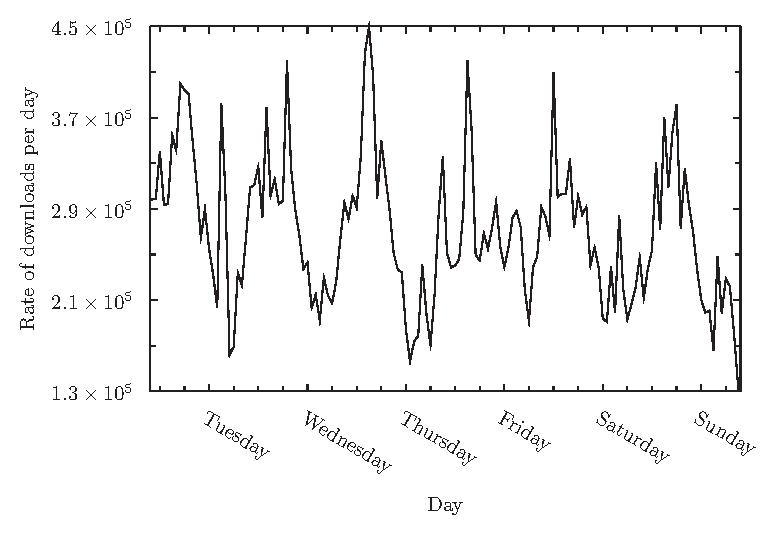
\includegraphics[width=\textwidth]{examples/eps/ex_apachelog.eps}}
}

